% questions.tex —— 1958 年·广东卷 · 题目内容片段（无答案）
% 由 tools/generate_projects.py 依来源总账自 1958/1958_广东_数学真题_试题.md 生成，勿手改（改源 MD 后重跑）


\gkpart{一}

\begin{question}
\gkti{1}求二项式 $(3+2x)^5$ 展开式中 $x^3$ 的系数。

\end{question}
\begin{question}
\gkti{2}求证：

\nopagebreak[4]
\[
\cos x\cdot\cos 2x\cdot\cos 4x=\frac{\sin 8x}{8\sin x}\qquad(x\ne k\pi,\ k\ \text{为任意整数})
\]

\Needspace{0.4\textheight}
\end{question}
\begin{question}
\gkti{3}$AB$、$AC$ 为 $\odot O$ 的两弦，$D$ 为 $\widehat{AB}$ 的中点，$E$ 为 $\widehat{AC}$ 的中点，连 $D$、$E$ 交 $AB$ 于 $M$，交 $AC$ 于 $N$。求证：$AM=AN$。
\nopagebreak[4]
\begin{center}% 1958 年广东卷第 3 题：⊙O 中弦 AB、AC，D 为弧 AB 中点、E 为弧 AC 中点，DE 交 AB 于 M、交 AC 于 N（按源卷布局）
\begin{tikzpicture}[scale=1.05, line width=0.45pt,
  every node/.style={inner sep=1.5pt}]
  \coordinate (O) at (0,0);
  \coordinate (A) at (-1.6,0);
  \coordinate (D) at (-0.55,1.5);
  \coordinate (E) at (-0.55,-1.5);
  \coordinate (B) at (1.13,1.13);
  \coordinate (C) at (1.13,-1.13);
  \coordinate (M) at (-0.55,0.44);
  \coordinate (N) at (-0.55,-0.44);
  \draw (O) circle (1.6);
  \draw (D) -- (E);
  \draw (A) -- (B);
  \draw (A) -- (C);
  \fill (A) circle (1.3pt);
  \fill (B) circle (1.3pt);
  \fill (C) circle (1.3pt);
  \fill (D) circle (1.3pt);
  \fill (E) circle (1.3pt);
  \fill (O) circle (1pt);
  \node[anchor=east] at (A) {$A$};
  \node[anchor=south] at (D) {$D$};
  \node[anchor=north] at (E) {$E$};
  \node[anchor=south west] at (B) {$B$};
  \node[anchor=north west] at (C) {$C$};
  \node[anchor=south west] at (M) {$M$};
  \node[anchor=north west] at (N) {$N$};
  \node[anchor=west] at (O) {$O$};
  % 角标 ∠1（M 处）、∠2（N 处），按源图 p-2 所标
  \draw (M) ++(-0.34,0.06) arc (170:262:0.26);
  \node[anchor=east] at ($(M)+(-0.30,0)$) {\tiny$1$};
  \draw (N) ++(-0.34,-0.06) arc (190:98:0.26);
  \node[anchor=east] at ($(N)+(-0.30,0)$) {\tiny$2$};
\end{tikzpicture}
\end{center}
\nopagebreak[4]
\Needspace{0.4\textheight}
\end{question}
\begin{question}
\gkti{4}求证：正四面体相对的两棱互相垂直。
\nopagebreak[4]
\begin{center}% 1958 年广东卷第 4 题：正四面体 ABCD，O' 为顶点 A 在底面 BCD 内的射影（按源卷布局；解析正文中记作 O，图中原卷标作 O'，转录保留原卷写法）
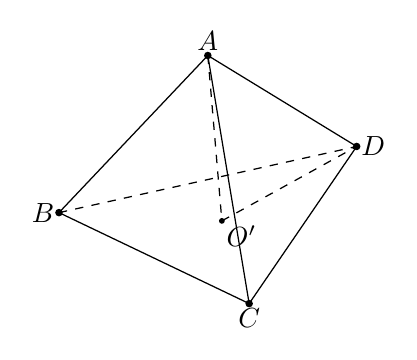
\begin{tikzpicture}[scale=1.05, line width=0.45pt,
  every node/.style={inner sep=1.5pt}]
  \coordinate (A) at (0,1.6);
  \coordinate (B) at (-1.8,-0.3);
  \coordinate (C) at (0.5,-1.4);
  \coordinate (D) at (1.8,0.5);
  \coordinate (Op) at (0.17,-0.4);
  \draw (A) -- (B);
  \draw (A) -- (C);
  \draw (A) -- (D);
  \draw (B) -- (C);
  \draw (C) -- (D);
  \draw[dashed] (B) -- (D);
  \draw[dashed] (A) -- (Op);
  \draw[dashed] (Op) -- (D);
  \fill (A) circle (1.3pt);
  \fill (B) circle (1.3pt);
  \fill (C) circle (1.3pt);
  \fill (D) circle (1.3pt);
  \fill (Op) circle (1pt);
  \node[anchor=south] at (A) {$A$};
  \node[anchor=east] at (B) {$B$};
  \node[anchor=north] at (C) {$C$};
  \node[anchor=west] at (D) {$D$};
  \node[anchor=north west] at (Op) {$O'$};
\end{tikzpicture}
\end{center}
\nopagebreak[4]
\end{question}
\begin{question}
\gkti{5}解方程 $\sin x=\sqrt3\cos x$。

\end{question}
\gkpart{二}

\begin{question}
\gkti{6}解方程组：

\nopagebreak[4]
\[
\begin{cases}
\sqrt{x+\dfrac1y}+\sqrt{x+2y-1}=4,\\[4pt]
2x+2y+\dfrac1y=9.
\end{cases}
\]

\end{question}
\gkpart{三}

\Needspace{0.4\textheight}
\begin{question}
\gkti{7}设有两个同心圆，半径各为 $R$、$r$（$R>r$）。今由圆心 $O$ 作半径交大圆于 $A$，交小圆于 $A'$，由 $A$ 作直线 $AD$ 垂直于大圆直径 $BC$，并交 $BC$ 于 $D$，作 $A'E\perp AD$，并交 $AD$ 于 $E$。

已知：$\angle OAD=\alpha$。

求：$OE$ 的长。
\nopagebreak[4]
\begin{center}% 1958 年广东卷第 7 题：同心圆 O（半径 R、r），半径 OA 交大圆于 A、交小圆于 A'，AD⊥BC 于 D，A'D'⊥BC 于 D'，A'E⊥AD 于 E（按源卷布局）
\begin{tikzpicture}[scale=1.0, line width=0.45pt,
  every node/.style={inner sep=1.5pt}]
  \coordinate (O) at (0,0);
  \coordinate (B) at (0,2);
  \coordinate (C) at (0,-2);
  \coordinate (D) at (0,-1.148);
  \coordinate (Dp) at (0,-0.631);
  \coordinate (A) at (-1.638,-1.148);
  \coordinate (Ap) at (-0.901,-0.631);
  \coordinate (E) at (-0.901,-1.148);
  \draw (O) circle (2);
  \draw (O) circle (1.1);
  \draw (B) -- (C);
  \draw (A) -- (D);
  \draw (O) -- (A);
  \draw (O) -- (E);
  \draw (Ap) -- (D);
  \draw[dashed] (Ap) -- (Dp);
  \draw (Ap) -- (E);
  \draw (A) ++(0:0.32) arc (0:35:0.32);
  \draw (Ap) ++(0:0.18) arc (0:35:0.18);
  \node[anchor=west] at ($(A)+(17:0.48)$) {$\alpha$};
  \node[anchor=south west] at ($(Ap)+(17:0.3)$) {\tiny$\alpha$};
  \fill (O) circle (1pt);
  \fill (A) circle (1.3pt);
  \fill (Ap) circle (1.3pt);
  \fill (D) circle (1.3pt);
  \fill (Dp) circle (1.3pt);
  \fill (E) circle (1.3pt);
  \fill (B) circle (1.3pt);
  \fill (C) circle (1.3pt);
  \node[anchor=south] at (B) {$B$};
  \node[anchor=north] at (C) {$C$};
  \node[anchor=east] at (O) {$O$};
  \node[anchor=north west] at (D) {$D$};
  \node[anchor=south west] at (Dp) {$D'$};
  \node[anchor=east] at (A) {$A$};
  \node[anchor=south east] at (Ap) {$A'$};
  \node[anchor=north] at (E) {$E$};
\end{tikzpicture}
\end{center}
\nopagebreak[4]
\end{question}
\gkpart{四}

\Needspace{0.4\textheight}
\begin{question}
\gkti{8}已知 $\triangle ABC$，求作圆过 $A$ 及 $AB$ 中点 $M$，并与 $BC$ 相切。
\nopagebreak[4]
\begin{center}% 1958 年广东卷第 8 题：△ABC 中过 A、AB 中点 M 且与 BC 相切于 T 的圆 O；辅助半圆（直径 AD，BD=BM，BE⊥AD 于 B，用以作比例中项 BE）（按源卷布局）
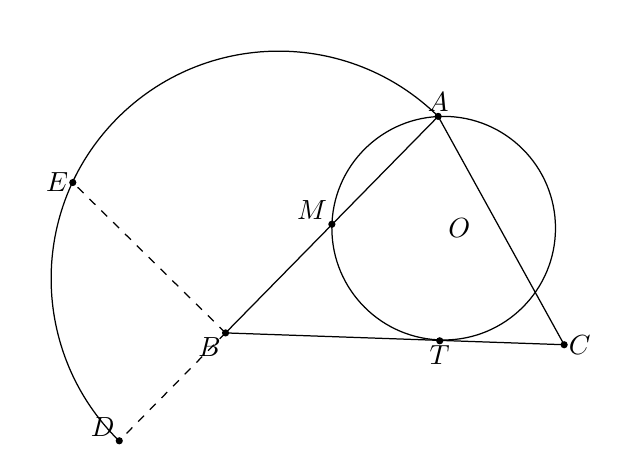
\begin{tikzpicture}[scale=1.0, line width=0.45pt,
  every node/.style={inner sep=1.5pt}]
  \coordinate (A) at (2.70,2.75);
  \coordinate (B) at (0,0);
  \coordinate (C) at (4.30,-0.15);
  \coordinate (M) at (1.35,1.38);
  \coordinate (O) at (2.77,1.33);
  \coordinate (T) at (2.72,-0.10);
  \coordinate (D) at (-1.35,-1.37);
  \coordinate (E) at (-1.94,1.91);
  \draw (A) -- (B) -- (C) -- cycle;
  \draw (O) circle (1.42);
  \draw[dashed] (B) -- (E);
  \draw[dashed] (B) -- (D);
  \draw (A) arc (45.5:225.5:2.89);
  \fill (A) circle (1.3pt);
  \fill (B) circle (1.3pt);
  \fill (C) circle (1.3pt);
  \fill (M) circle (1.3pt);
  \fill (T) circle (1.3pt);
  \fill (D) circle (1.3pt);
  \fill (E) circle (1.3pt);
  \node[anchor=south] at (A) {$A$};
  \node[anchor=north east] at (B) {$B$};
  \node[anchor=west] at (C) {$C$};
  \node[anchor=south east] at (M) {$M$};
  \node[anchor=west] at (O) {$O$};
  \node[anchor=north] at (T) {$T$};
  \node[anchor=south east] at (D) {$D$};
  \node[anchor=east] at (E) {$E$};
\end{tikzpicture}
\end{center}
\nopagebreak[4]
\end{question}
\gkpart{五}

\Needspace{0.4\textheight}
\begin{question}
\gkti{9}已知一直角三角形的斜边长为 $2$，斜边上的高为 $\dfrac{\sqrt3}{2}$，求证：此三角形的两个锐角是下列三角方程的根：

\nopagebreak[4]
\[
\sin^2x-\frac{1+\sqrt3}{2}\sin x+\frac{\sqrt3}{4}=0
\]
\nopagebreak[4]
\begin{center}% 1958 年广东卷第 9 题：直角三角形，斜边 2，斜边上的高 √3/2，两腰记 a、b，右侧锐角记 α（按源卷布局）
\begin{tikzpicture}[scale=1.6, line width=0.45pt,
  every node/.style={inner sep=1.5pt}]
  \coordinate (L) at (0,0);
  \coordinate (R) at (2,0);
  \coordinate (F) at (0.5,0);
  \coordinate (P) at (0.5,0.866);
  \draw (L) -- (R) -- (P) -- cycle;
  \draw (P) -- (F);
  \draw (F) ++(0,0.08) -- ++(0.08,0) -- ++(0,-0.08);
  \node[anchor=south east] at (0.14,0.50) {$a$};
  \node[anchor=west] at ($(P)!0.5!(R)$) {$b$};
  \node[anchor=north] at ($(L)!0.5!(R)$) {$2$};
  \node[anchor=west] at (0.56,0.42) {$\dfrac{\sqrt3}{2}$};
  \node[anchor=north west] at (1.68,0.05) {$\alpha$};
\end{tikzpicture}
\end{center}
\nopagebreak[4]

\end{question}